\chapter{Instrukcja użytkownika}

\section{Wersja Pordukcyjna}
Wersja produkcyjna aplikacji jest uruchomiona na serwerze heroku, pod adresem \url{http://terrain-editor.herokuapp.com}{http://terrain-editor.herokuapp.com}

Pierwsze uruchomienie wymaga uruchomienia serwera, który przechodzi w stan uśpienia po godzinie braku aktywności ze strony użytkowników w celu oszczędności zasobów. Z tego powodu po wpisaniu adresu w przeglądarce internetowej po raz pierwszy, należy zaczekać nieco dłużej niż w przypadku kolejnych zapytań do serwera.

\subsection{Logowanie i rejestracja}
Aby mieć dostęp do wszystkich funkcji aplikacji, należy się zalogować, lub zarejestrować nowego użytkownika.

Ze względu na przeznaczenie projektu do celów edukacyjnych, postanowiłem nie walidować adresów email pod kątem prawdziwości, dlatego dopuszczalne do rejestracji są fałszywe adresy, pod warunkiem że zachowany zostanie poprawny format.

W wersji pokazowej zarejestrowany został użytkownik:
\textbf{email:} test.user@example.com
\textbf{hasło:} password

\FloatBarrier
 	\begin{figure}[ht]
        \centering
        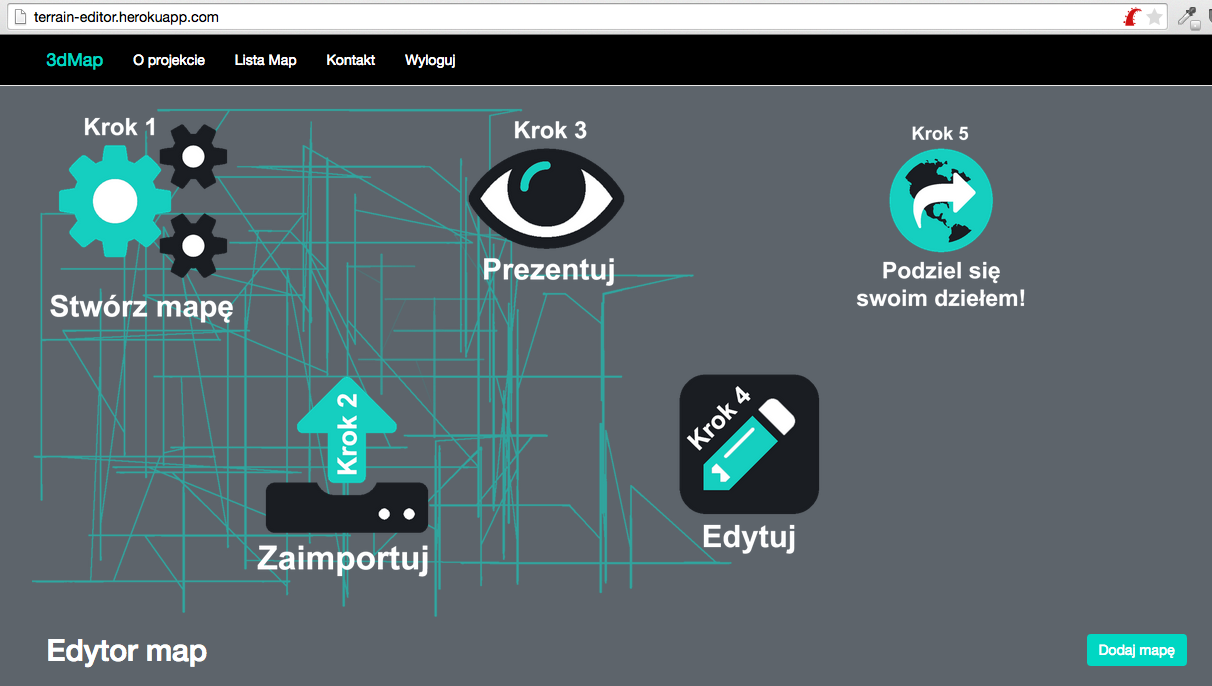
\includegraphics[width=0.90\textwidth,height=0.46\textheight]{img/home.png}
	\caption{Strona główna aplikacji}
        \label{rys:screen_home}
    \end{figure}
\FloatBarrier
	
\subsection{Kontrola dostępu}

Wykorzystanie sesji logowania pozwoliło na ograniczenie praw dla użytkowników niezalogowanych, jak i dla zalogowanych.

\begin{itemize}
\item Użytkownicy niezalogowani mogą:
	\subitem Przeglądać mapy
	\subitem Logować się, i rejestrować
	\subitem Wysyłać emaile kontaktowe
			
\item Użytkownicy zalogowani mogą:
	\subitem Wykonywać wszystkie akcje niezalogowanych użytkowników z wyjątkiem rejestracji i logowania.
	\subitem Dodawać mapy
	\subitem Edytować swoje mapy
\end{itemize}

W przypadku próby wykonania akcji zabronionej, użytkownik niezalogowany jest przekierowywany do ekranu logowania, zaś zalogowany użytkownik do strony głównej.

Na górze ekranu pojawi się wiadomość o braku uprawnień do wykonania danej akcji.

\FloatBarrier
 	\begin{figure}[ht]
        \centering
        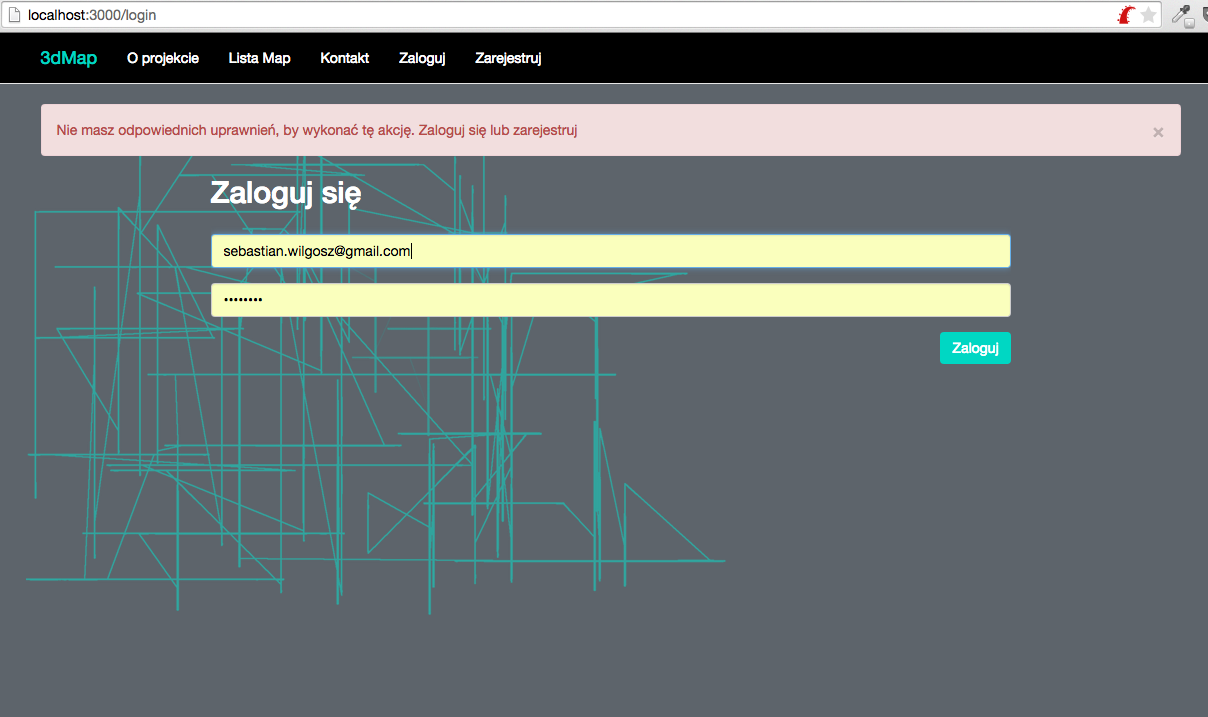
\includegraphics[width=0.90\textwidth,height=0.46\textheight]{img/no_access.png}
	\caption{Próba wykonania akcji zabronionej}
        \label{rys:screen_no_access}
    \end{figure}
\FloatBarrier


\section{Wersja lokalna}

ubuntu/reverse
